\documentclass[12pt,a4paper,openany]{book}

\input{C:/Users/serru/Documents/Codes/LaTeX/Environnement_package.tex}
\input{C:/Users/serru/Documents/Codes/LaTeX/Environnements_settings.tex}
\input{C:/Users/serru/Documents/Codes/LaTeX/Environnement_theorems.tex}

\setcounter{tocdepth}{4}
\sloppy

\title{}
\author{Serrurot Gabin\\
BTS SNIR}
\date{\today}

\begin{document}

\sloppy

\vspace*{\stretch{1}}
\begin{minipage}{0.9\linewidth}
\rule{\linewidth}{0.5mm}\\[0.2cm]
\huge\bfseries
\begin{center}
Physique S1
\end{center}
\rule{\linewidth}{0.5mm}\\[0.2cm]
\maketitle
\end{minipage}
\vspace*{\stretch{1}}

\newpage

\tableofcontents

\newpage

\chapter{Théorèmes généraux sur les circuits}

\section{Introduction}

Nous avons la relation:
\begin{equation}
I = \frac{Q}{\Delta t} = \frac{Nq_{e}}{\Delta t} \text{\hspace{20px} avec $q_{e} = -1.60.10^{-19}$ C.}
\end{equation}

Elle définie l'intensité du courant électrique (en Ampères) en fonction de la quantité de courant (en Coulombs) par unités de temps (en secondes).

\section{Loi des nœuds}

Par convention, le courant circule de la borne \textbf{+} vers la borne \textbf{-} (ou le \textbf{COM}). Il circule donc vers les potentiels les plus bas.\\
Un ampèremètre se branche de sorte que le courant le traverse d'abord par sa borne \textbf{+} vers sa borne \textbf{-} (ou le \textbf{COM}). Le courant doit donc circuler de la même manière que circule le courant dans un circuit.\\
Nous pouvons donc définir la notion de nœud. En effet, on parle de nœud lorsque dans un circuit, il y a un point qui relie 3 fils. La loi de conservation de la charge impose que la quantité d'électrons rentrant dans un nœud soit égale à la quantité d'électrons sortant. On obtient donc la loi des nœuds:
\begin{Definition}
La somme des intensités des courants rentrant dans un nœud est égale à la somme des intensités des courant sortant de ce nœud.
\end{Definition} 

\section{Loi des mailles}

Nous pouvons définir la notion de potentiel en tout point du circuit. Ainsi, nous pouvons obtenir une différence de potentiels (donc une tension qui est une grandeur algébrique) entre deux points. Ainsi, une tension entre le point A et le point B sera notée $ U_{AB} $ et sera fléchée de B vers A.\\
Comme un ampèremètre, le voltmètre se branche de sorte que le courant circule du \textbf{+} vers le \textbf{-} (ou le \textbf{COM}). Ainsi, la borne \textbf{+} du voltmètre se place au point A et la borne \textbf{-} du voltmètre se branche au point B.\\
Nous pouvons définir la notion de maille. En effet, une maille est une portion du circuit qui est constituée de plusieurs branches formant un circuit fermé. Ainsi, en choisissant un sens de parcours arbitraire dans cette maille, nous pouvons dire :
\begin{Definition}
La somme algébrique des tensions à l'intérieur d'une maille est nulle.
\end{Definition} 

\newpage

\section{Loi d'Ohm}

Nous pouvons définir deux conventions pour un dipôle:
\begin{itemize}
\item la convention générateur: c'est lorsque les flèches de tension et l'intensité vont dans le même sens
\item la convention récepteur: c'est lorsque les flèches de tension et l'intensité vont dans le sens contraire
\end{itemize}

Il faut donc adapter le sens des flèches au dipôle: une résistance sera en convention récepteur et un générateur sera en convention générateur.\\
Nous pouvons donc définir la loi d'Ohm en convention récepteur:
\begin{equation}
U = RI \text{\hspace{20px} en convention récepteur}
\end{equation}
\begin{equation}
U = -RI \text{\hspace{20px} en convention générateur}
\end{equation}

\section{Association de résistances}

Nous pouvons associer les résistances d'un montage pour obtenir une résistance équivalente. Nous avons donc deux cas possibles:
\begin{figure}[!h]
\begin{center}
\subfloat[Schéma d'un montage de résistances en série.]{
\label{montageSerie}
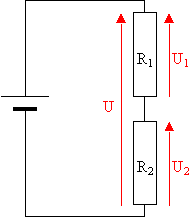
\includegraphics[scale=1]{Images/resistancesSerie.png} }
\hfill
\subfloat[Schéma d'un montage de résistances en dérivation.]{
\label{montageDerivation}
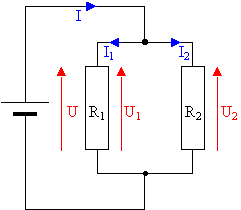
\includegraphics[scale=1]{Images/resistancesderivation.png} }
\end{center}
\caption{}
\end{figure}


Si les résistances sont montées en série comme dans le montage~\ref{montageSerie} ci-dessus, alors en faisant une loi des mailles nous obtenons la relation suivante:
\begin{equation}
R_{eq} = \Sigma R_{i}
\end{equation}

Si les résistances sont montées en dérivation comme dans le montage~\ref{montageDerivation} ci-dessus, alors en faisant une loi des mailles nous obtenons la relation suivante:
\begin{equation}
\frac{1}{R_{eq}} = \Sigma\frac{1}{R_{i}}
\end{equation}

\newpage

\section{Pont diviseur de tensions}

Nous pouvons parler de pont diviseur de tension lorsque des résistances sont montées en série. Nous avons donc le schéma ci-dessous:
\begin{figure}[!h]
\begin{center}
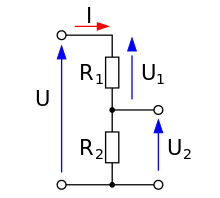
\includegraphics[scale=1]{Images/pontDiviseurTension.png} 
\caption{Schéma d'un montage de pont diviseur de tension.}
\label{pontDiviseurTension}
\end{center}
\end{figure}

Nous avons donc la relation suivante:
\begin{equation}
U_{2} = \frac{R_{2}}{\Sigma R_{i}}U
\end{equation}

\section{Puissances et énergie électrique}

Nous pouvons définir la puissance électrique reçue par un dipôle:\\
\begin{equation}
P = UI
\label{relationPuissance}
\end{equation}

De plus, nous savons que la tension et l'intensité électrique sont des grandeurs algébrique donc la puissance l'est aussi. Ainsi, nous pouvons déduire deux cas:
\begin{itemize}
\item P > 0 : le dipôle reçoit de la puissance, il est donc \textbf{récepteur}
\item P < 0 : le dipôle perd de la puissance, il est donc \textbf{générateur}
\end{itemize}

Cette puissance se mesure avec un wattmètre qui mesure à la fois le courant et la tension afin d'en déduire la puissance. Il possède donc 4 bornes.\\
Ainsi, un dipôle donné ne peut pas admettre autant d'énergie qu'il le souhaite, il y a une limite maximale. Nous pouvons donc utiliser la relation~\ref{relationPuissance} pour calculer la tension maximale ou le courant maximal qui traverse un dipôle pour ne pas l'endommager. En fonction de la contrainte soit sur la tension, soit sur l'intensité du courant, nous avons deux équations possibles (les deux se déduire en injectant la loi d'Ohm dans l'équation sur la puissance électrique):
\begin{equation}
P = RI^{2} = \frac{U^{2}}{R}
\end{equation}

La puissance calculée est donc la puissance maximale à utiliser. Si on dépasse cette valeur, le composant pourrait être endommagé.

\newpage

Nous pouvons relier cette notion de puissance maximale à la notion d'énergie maximale:
\begin{align}
E = P\Delta t \Rightarrow E = RI^{2} = \frac{U^{2}}{R} \Rightarrow E = P_{j}\Delta t
\end{align}

$ P_{j} $ est la puissance de Joule. Ainsi, on a la même relation qu'en mécanique, mais avec la puissance qui est définie comme précédemment.

\begin{figure}[!h]
\begin{center}
\begin{tikzpicture}
\draw[thin][->] (0, 0) -- (3, 0);
\draw[thin] (3, -0.5) -- (3, 0.5) -- (6, 0.5) -- (6, -0.5) -- (3, -0.5);
\draw[thin][->] (6, 0) -- (9, 0);
\draw[thin][->] (4.5, -0.5) -- (5.5, -1);
\draw (1.5,0) node[above] {$P_{entree}$};
\draw (7.5,0) node[above] {$P_{sortie}$};
\draw (5.5,-1) node[right] {$P_{pertes}$};
\end{tikzpicture}
\end{center}
\end{figure}

Nous pouvons noter que les puissances s'ajoutent de la même manière que la loi des nœuds:
\begin{equation}
P_{entree} = P_{sortie} + P_{pertes}
\end{equation}

Nous pouvons également définir le rendement:
\begin{equation}
\eta = \frac{P_{sortie}}{P_{entree}}
\end{equation}

\chapter{Les grandeurs périodiques: généralités}

Les grandeurs dépendant du temps seront notées en minuscules. Nous parlerons donc d'une grandeur à un instant donné. Nous parlerons par exemple d'une intensité de $ 20 mA $ à $ t = 80 \mu s $.

\section{Les grandeurs périodiques}

Derrière la notion de périodicité d'une fonction se cachent diverses informations.

\paragraph{La période} C'est la durée minimale nécessaire pour qu'un motif se répète. Elle est notée \textbf{T} et nous étudierons donc nos signaux sur une unique période.

\paragraph{La fréquence} C'est le nombre de périodes contenues dans une durée égale à $ 1s $. Nous pouvons la calculer en faisant:
\begin{equation}
f = \frac{1}{T}
\end{equation}

\paragraph{Les valeurs extrémales} Ce sont les valeurs de la plus haute image ainsi que de la plus basse. Ces deux grandeurs peuvent nous renseigner sur la tension crête-à-crête par exemple.

\paragraph{La valeur moyenne} Elle correspond à la surface relative contenue entre la courbe et l'axe des abscisses. Nous avons donc la relation:
\begin{equation}
<X> = \frac{\Sigma A_{i}}{T}
\end{equation}

Nous pouvons donc appliquer la méthode suivante:
\begin{enumerate}
\item tout d'abord on identifie la période
\item ensuite nous découpons cette période en formes géométriques simples
\item après ceci nous calculons l'aire de toutes ces formes géométriques
\item enfin nous faisons la somme de toutes et après nous divisons le résultat par une période
\end{enumerate}

Nous pouvons rajouter que la moyenne est indépendante de la période, qu'elle peut être appelée \textbf{composante continue} et que si elle est nulle alors le signal est \textbf{alternatif}.

\paragraph{La valeur efficace} 
\begin{Definition}
La valeur efficace d'une grandeur périodique est la valeur qu'il faudrait donner à une grandeur constante pour fournir la même puissance à une résistance.
\end{Definition} 

La valeur efficace est toujours notée en majuscule. Elle est définit par la relation:
\begin{equation}
X = \sqrt{< x^{2} >}
\label{relationGrandeurEfficace}
\end{equation}

Nous pouvons donc la calculer selon la méthode suivante:
\begin{enumerate}
\item on élève la grandeur au carré
\item on calcule la valeur moyenne de cette valeur au carré
\item on prend la racine du résultat
\end{enumerate}

Si par exemple nous avons comme signal une fonction rectangle, nous faisons comme ceci:
\begin{figure}[!h]
\begin{center}
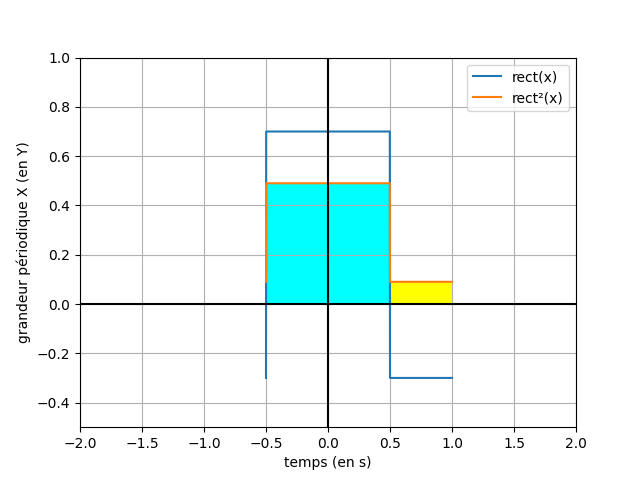
\includegraphics[scale=0.8]{Images/grapheAuCarre.png} 
\caption{Graphique montrant une période de la fonction $ rect(x) $ ainsi que sa mise au carré.}
\label{grapheFonctionMiseAuCarre}
\end{center}
\end{figure}

Sur le graphique~\ref{grapheFonctionMiseAuCarre}, nous avons tracé un signal mis au carré; ceci représente la première étape de la méthode précédente. La deuxième étape consiste donc à calculer la moyenne de la courbe au carré:
\begin{align*}
<X^{2}> & = \frac{A_{bleue} + A_{jaune}}{T}\\
	& = \frac{(0.5 - (-0.5))*0.7^{2} + (1 - 0.5)*(-0.3)^{2}}{1.5}\\
	& \approx 0.36~Y^{2}
\end{align*}

Nous pouvons à présent calculer la grandeur efficace:
\begin{align*}
X 	& = \sqrt{<X^{2}>}\\
	& = \sqrt{0.36}\\
	& = 0.6~Y
\end{align*}

\newpage

\section{Composantes continue et variable}

En physique, nous avons souvent ce genre de signal (en bleu):
\begin{figure}[!h]
\begin{center}
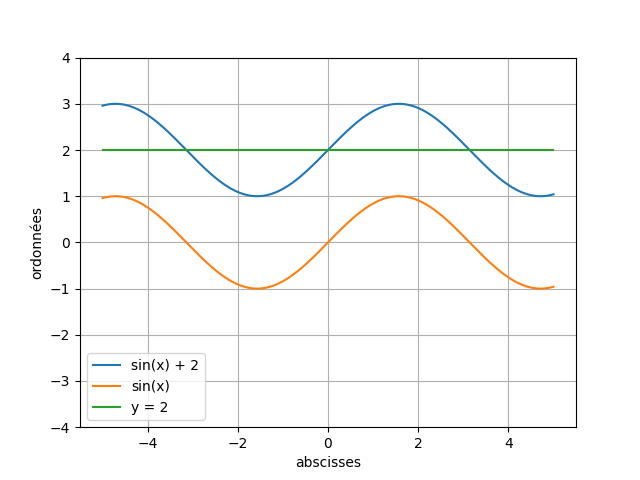
\includegraphics[scale=0.8]{Images/composanteVariableContinue.png} 
\caption{Graphique représentant un signal quelconque (ici en bleu) comme étant la somme de deux autres signaux (ici en vert et en orange).}
\label{composanteVariableContinue}
\end{center}
\end{figure}

Ce genre de signal peut souvent être décomposé en une somme de signal alternatif (en orange) et continue (en vert). En effet, les signaux périodiques sont soit alternatifs (donc leur moyenne est nulle), soit leur moyenne est différente de zéro. Cependant, un signal périodique peut être plus ou moins monté ou descendu pour avoir une moyenne nulle: c'est ce qui est représenté dans la figure~\ref{composanteVariableContinue}. Nous avons donc la relation suivante:
\begin{equation}
U^{2}_{eff} = <U>^{2} + U^{2}_{ac}
\end{equation}

Nous avons donc, dans le cas de la figure~\ref{composanteVariableContinue}:
\begin{equation*}
\textcolor{blue}{U_{eff}}^{2} = \textcolor{green}{2}^{2} + \textcolor{orange}{U_{ac}}^{2}
\end{equation*}

La valeur moyenne d'un signal \textbf{alternatif} ou \textbf{non alternatif} se mesure avec un appareil en mode \textbf{DC}.\\
La valeur efficace d'un signal \textbf{alternatif} ou \textbf{non alternatif} se mesure toujours avec un appareil en mode \textbf{AC+DC}. Cependant, si le signal est \textbf{alternatif}, nous pouvons nous contenter du mode \textbf{AC}. Nous pouvons voir les choses selon la relation (qui est vraie \textbf{du point de vue des appareils}):
\begin{equation*}
U^{2}_{AC+DC} = U^{2}_{DC} + U^{2}_{AC}
\end{equation*}

\newpage

\section{Application}

Nous avons le graphique suivant:
\begin{figure}[!h]
\begin{center}
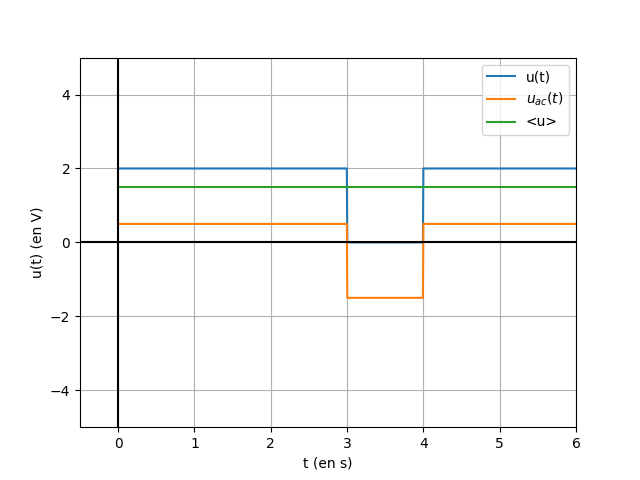
\includegraphics[scale=0.8]{Images/applicationChapitre2.png} 
\caption{Graphique représentant une tension en fonction du temps.}
\label{applicationChapitre2}
\end{center}
\end{figure}

\begin{itemize}
\item La grandeur $ u(t) $ est-elle alternative ?\\
\textcolor{red}{Non car la moyenne n'est pas nulle.}
\item Calculer la valeur moyenne $ <u> $ de $ u(t) $. Comment mesurer cette valeur ?\\
\textcolor{red}{
\begin{align*}
<u> & = \frac{2.\frac{3T}{4}}{T}\\
	& = 1.5~V
\end{align*}
Pour mesurer ceci, nous utiliserons un voltmètre en mode DC.}
\item Décomposer $ u(t) $ en une somme d'un signal continu et d'un signal alternatif.\\
\textcolor{red}{La décomposition est faite sur la figure~\ref{applicationChapitre2}. La composante continue est la courbe verte et la composante alternative est la courbe orange.}
\item Calculer la valeur moyenne $ <u_{ac}> $ de $ u_{ac}(t) $. Ce signal est-il alternatif ?\\
\textcolor{red}{
\begin{align*}
<u_{ac}> & = \frac{0.5\frac{3T}{4} + (-1.5)\frac{T}{4}}{T}\\
		 & = \frac{3}{8} - \frac{3}{8}\\
		 & = 0~V
\end{align*}
Ce signal est donc alternatif.
}
\item Calculer la valeur efficace $ U_{ac} $ de $ u_{ac}(t) $. Comment mesurer cette valeur ?\\
\textcolor{red}{
\begin{align*}
U_{ac} & = \sqrt{\frac{0.5^{2}\frac{3T}{4} + (-1.5)^{2}\frac{T}{4}}{T}}\\
	   & \approx 0.87~V
\end{align*}
Pour mesurer ceci, nous utiliserons un voltmètre en mode AC+DC? Nous pouvons aussi utiliser le mode AC en alternatif.}
\item Calculer la valeur efficace $ U $ de $ u(t) $. Comment mesurer cette valeur ?\\
\textcolor{red}{
\begin{align*}
U^{2} & = <U>^{2} + U^{2}_{ac}\\
\Rightarrow U & = \sqrt{<U>^{2} + U^{2}_{ac}}\\
			  & = \sqrt{3}~V
\end{align*}
Nous pouvons uniquement utiliser un voltmètre en mode AC+DC.
}
\end{itemize}

\section{Propriété énergétique}

Nous avons 3 sortes de puissances:

\paragraph{Puissance instantanée p(t)} Elle correspond à la puissance instantanée transportée par un signal. Elle est définie par:
\begin{equation}
p(t) = u(t)i(t)
\end{equation}

\begin{itemize}
\item en convention récepteur:
\begin{itemize}
\item si $ p(t)>0 $, le dipôle \textbf{consomme} de la puissance
\item si $ p(t)<0 $, le dipôle \textbf{fourni} de la puissance
\end{itemize}
\item en convention générateur:
\begin{itemize}
\item si $ p(t)>0 $, le dipôle \textbf{fourni} de la puissance
\item si $ p(t)<0 $, le dipôle \textbf{consomme} de la puissance
\end{itemize}
\end{itemize}

\paragraph{Puissance active P} Elle correspond à la puissance moyenne $ <p(t)> $ et se mesure avec un wattmètre. Elle vaut:
\begin{itemize}
\item en régime continu:
\begin{equation}
P = UI
\end{equation}
\item si la tension est constante et le courant est variable:
\begin{equation}
P = E<i>
\end{equation}
\item en régime sinusoïdal:
\begin{equation}
P = UIcos(\phi)
\end{equation}
\end{itemize}

\paragraph{Puissance apparente S} Elle s'exprime en (V.A) est définie par la relation:
\begin{equation}
S = UI
\end{equation}

U et I représentent la valeur efficace respectivement de $ u(t) $ et $ i(t) $.

\paragraph{Facteur de puissance} Le facteur de puissance est défini par la relation:
\begin{equation}
k = \frac{P}{S}
\end{equation}

\paragraph{Puissance réactive} La puissance réactive se définie selon la relation suivante:
\begin{equation}
Q = \sqrt{S^{2} - P^{2}}
\end{equation}

Prenons le cas suivant:
\begin{figure}[!h]
\begin{center}
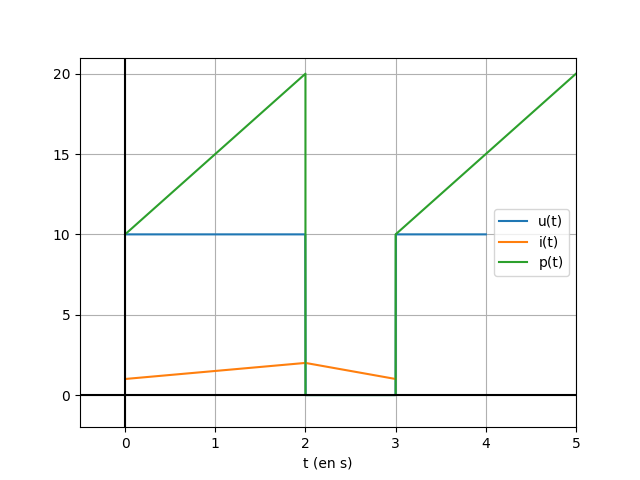
\includegraphics[scale=0.8]{Images/calculPuissance.png} 
\caption{Graphique montrant la composition d'une puissance instantanée.}
\label{calculPuissance}
\end{center}
\end{figure}

Dans ce cas, nous avons les valeurs suivantes:
\begin{itemize}
\item $ U = 8.16~V $
\item $ I = 1.52~A $
\item $ S = 12~V.A $
\item $ P = 10~W $
\item $ k \approx 0.83 $
\item $ Q = 8.8~W $
\end{itemize}

\chapter{Régime sinusoïdal alternatif: généralités}

\section{Grandeurs relatives au régime sinusoïdal}

Un signal est alternatif si son \textbf{équation horaire} est de la forme:
\begin{align}
u(t) & = U_{max}sin(\omega t + \theta_{u})\\
	 & = U\sqrt{2}sin(\omega t + \theta_{u}) \text{\hspace{20px} avec $ U $ la valeur efficace}
\end{align}

Cependant, il faut faire très attention car la relation $ U_{max} = U\sqrt{2} $ n'est \textbf{vraie} que pour une \textbf{sinusoïde alternative}. Cette fonction se représente donc par le graphe suivant:
\begin{figure}[!h]
\begin{center}
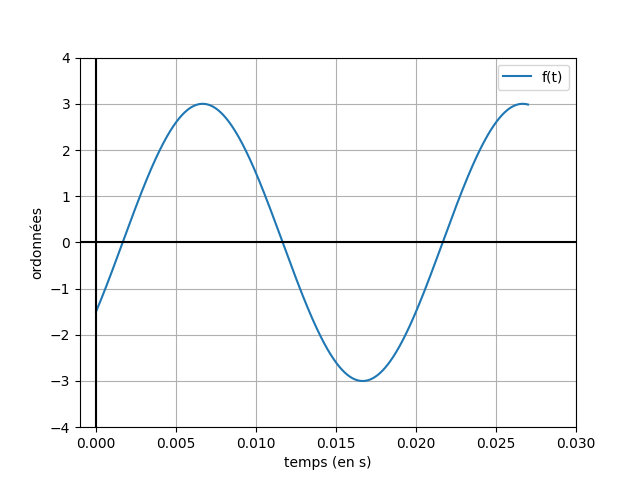
\includegraphics[scale=0.8]{Images/representationSinusoideGeneralites.png} 
\caption{Graphique représentant une tension en régime sinusoïdal.}
\label{representationSinusoideGeneralites}
\end{center}
\end{figure}

Nous avons donc $ \omega = \dfrac{2\pi}{T} $ (ici $ \omega = 314~rad.s^{-1} $). Par lecture graphique, nous pouvons voir que $ U_{max} = 3~V $. Pour l'instant, notre équation horaire de la sinusoïde du graphe~\ref{representationSinusoideGeneralites} est donc:
\begin{equation*}
u(t) = 3sin(314t + \theta)
\end{equation*}

Nous devons désormais déterminer la phase à l'origine. Nous avons:
\begin{align*}
u(t) & = 3sin(314t + \theta)\\
u(t=0) & = 3sin(\theta)\\
\Leftrightarrow -1.5 & = 3sin(\theta) \text{\hspace{20px} le $ 1.5~V $ est lu graphiquement}\\
\Leftrightarrow \theta & = arcsin\left(\dfrac{-1.5}{3}\right)\\
					   & = arcsin\left(-0.5\right)\\
					   & = \{\dfrac{-\pi}{6}; \dfrac{-5\pi}{6}\}
\end{align*}

Deux solutions sont possibles:
\begin{equation*}
u(t) = 3sin\left(314t - \dfrac{\pi}{6}\right) \text{\hspace{20px} ou \hspace{20px}} u(t) = 3sin\left(314t - \dfrac{5\pi}{6}\right)
\end{equation*}

Pour déterminer la bonne solution, nous allons utiliser la \textbf{représentation vectorielle de Fresnel}. Une très bonne animation se trouve sur \href{https://phyanim.sciences.univ-nantes.fr/Elec/Alternatif/Fresnel_FJ.php}{\textcolor{blue}{ce site}}. Nous avons donc deux solutions:
\begin{figure}[!h]
\begin{center}
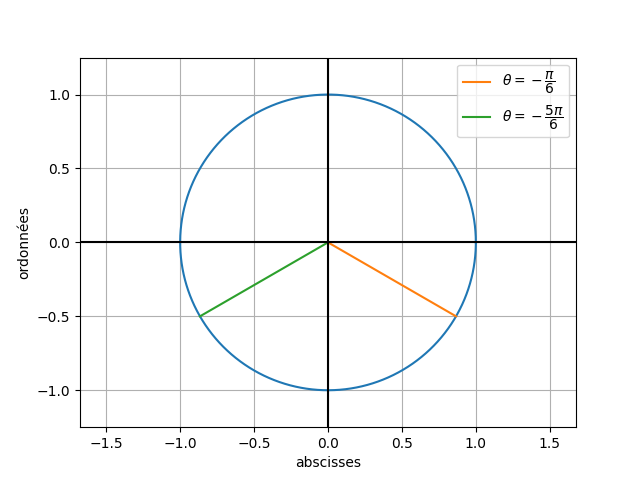
\includegraphics[scale=0.8]{Images/fresnelSinusoideGeneralites.png} 
\caption{Représentation de Fresnel de la situation précédente.}
\label{fresnelSinusoideGeneralites}
\end{center}
\end{figure}

Grâce à l'animation et à la figure~\ref{fresnelSinusoideGeneralites} qui montre les deux solutions possibles, nous pouvons déduire que, puisque le graphe~\ref{representationSinusoideGeneralites} est \textbf{croissant} en partant de l'\textbf{origine}, la bonne solution est:
\begin{align*}
u(t) & = 3sin\left(314t - \dfrac{\pi}{6}\right)\\
	 & = 2.1\sqrt{2}sin\left(314t - \dfrac{\pi}{6}\right)
\end{align*}

Nous pouvons également représenter ce signal par sa \textbf{notation complexe}. En effet, puisqu'un nombre complexe avec la \textbf{notation trigonométrique} est défini par son \textbf{module} et son \textbf{argument}, nous avons dans ce cas $ U = 2.1~V $ et $ \theta = -\dfrac{\pi}{6} $ donc nous avons:
\begin{equation*}
\underline{U} = \left[2.1; -\dfrac{\pi}{6}\right]
\end{equation*}

\section{Notion de puissance en régime sinusoïdal}

Dans cette partie, nous allons faire une comparaison entre les différentes puissances en régime périodique et en régime sinusoïdal alternatif:
\begin{table}[!h]
\begin{center}
\begin{tabular}{|l|c|c|c|} %c/l/r pour centré/à gauche/droite
\hline type de grandeur & unité & Régime périodique & régime sinusoïdal alternatif\\
\hline Puissance active P & $ W $ & $ P  = <p(t)> = <u(t)i(t)> $ & $ P = UIcos(\theta_{u/i}) $\\
\hline Puissance apparente S & $ V.A $ & $ S = UI $ & $ S = UI $\\
\hline Puissance réactive Q & $ Var $ & $ Q = \sqrt{S^{2} - P^{2}} $ & $ Q = UIsin(\theta_{u/i}) $\\
\hline Facteur de puissance k &  & $ k = \dfrac{P}{S} $ & $ k = cos(\theta_{u/i}) $\\
\hline
\end{tabular}
\caption{Comparaison entre les méthodes de calculs de puissance en fonction du régime périodique étudié.}
\label{tableauComparaisonPuissances}
\end{center}
\end{table}

\end{document}